\section{不可约仿射簇}\label{sec:irreducible-affine-varieties}

现在来到本章的核心, 也是代数几何中的一个中心概念: 不可约性. 为了引出这一概念, 考虑仿射簇
\[
  X_{1}=\mathcal{V}(y-x^{2}),\quad X_{2}=\mathcal{V}(y-2),
  \quad\text{以及}\quad X_{3}=\mathcal{V}(x-1,y-3).
\]
\BookPairedFigure
  {$\mathbb{R}$ 上的仿射簇 $X=X_{1}\cup X_{2}\cup X_{3}$ 画在\hyperref[fig:three-irreducible-pieces]{右边}. 设想只给你看这幅图, 却不告诉你 $X$ 是三个仿射簇的并. 你很可能仍能从图上看出 $X$ 是这样的并, 仔细看图甚至可能确定这三个簇.}
  {\phantomsection\label{fig:three-irreducible-pieces}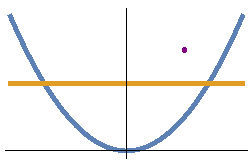
\includegraphics[width=\linewidth]{figures/three-irreducible-pieces.pdf}}
\noindent 这些簇是 $X$ 的基本组成部分, 即它的不可约分支.

如上所述, 把仿射簇分解成各个组成部分, 就是把它写成有限多个较小仿射簇的并. 因此, 基本组成部分正是那些不能写成两个较小仿射簇之并的仿射簇. 下面的定义把这一概念精确化.

\begin{Definition}{可约与不可约仿射簇}\leavevmode\label{def:reducible-and-irreducible-affine-varieties}
  若对某些仿射簇 $X_{1},X_{2}\subsetneq X$, 有 $X=X_{1}\cup X_{2}$, 则称仿射簇 $X\subseteq\mathbb{A}^{n}$ 是\textbf{可约的}. 若 $X$ 既非空也不是可约的, 则称它是\textbf{不可约的}.
\end{Definition}

\begin{Example}{}\leavevmode\label{ex:two-lines-reducible-variety}
  仿射簇 $X=\mathcal{V}(x^{2}-y^{2})\subseteq\mathbb{A}^{2}_{\mathbb{C}}$ 是可约的. 为见此点, 注意
  \[
    X=\mathcal{V}((x+y)(x-y))=\mathcal{V}(x+y)\cup\mathcal{V}(x-y).
  \]
  \BookPairedFigure
    {因此, 两个仿射簇
    \[
      X_{1}=\mathcal{V}(x+y)\subsetneq X
    \]
    与
    \[
      X_{2}=\mathcal{V}(x-y)\subsetneq X
    \]
    满足 $X=X_{1}\cup X_{2}$.}
    {\phantomsection\label{fig:two-crossing-lines}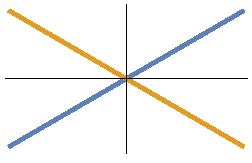
\includegraphics[width=\linewidth]{figures/two-crossing-lines.pdf}}
  \noindent 限制到实数时, 由\hyperref[fig:two-crossing-lines]{上图}可见, $X_{1}$ 和 $X_{2}$ 是构成 $X$ 的两条直线. 实际上, 如下一节将看到的, 簇 $X_{1}$ 和 $X_{2}$ 是 $X$ 的唯一两个不可约分支.
\end{Example}

\begin{Example}{}\leavevmode\label{ex:parabola-geometrically-irreducible}
  相比之下, 抛物线 $X=\mathcal{V}(y-x^{2})\subseteq\mathbb{A}^{2}$ 是不可约的. 从几何上看, 这个断言应当是可信的: 与 Example~\ref{ex:two-lines-reducible-variety} 中的仿射簇不同, 抛物线只由一\textquotedbl{}块\textquotedbl{}组成. 虽然这一直觉还不是证明, 但 $X$ 的不可约性可由下面的 Proposition~\ref{prop:irreducible-iff-vanishing-ideal-prime} 得出.
\end{Example}

如上面的例子所示, 证明仿射簇 $X$ 可约很直接: 找到一对仿射簇 $X_{1}\subsetneq X$ 和 $X_{2}\subsetneq X$, 使两者的并为 $X$. 怎样证明仿射簇不可约则没有那么明显. 下面用代数方法刻画不可约性, 提供一个关键工具.

\begin{Proposition}{不可约性的代数刻画}\leavevmode\label{prop:irreducible-iff-vanishing-ideal-prime}
  仿射簇 $X\subseteq\mathbb{A}^{n}$ 是不可约的, 当且仅当 $\mathcal{I}(X)$ 是素理想.
\end{Proposition}

\begin{Proof}
  我们分别证明两个方向的逆否命题.

  ($\Leftarrow$) 假设 $X$ 可约, 选取仿射簇 $X_{1},X_{2}\subsetneq X$, 使得
  \[
    X=X_{1}\cup X_{2}.
  \]
  因为 $X_{1}\subsetneq X$, 由 Proposition~\ref{prop:operators-reverse-inclusions} 得 $\mathcal{I}(X_{1})\supsetneq\mathcal{I}(X)$. 因此, 存在 $f\in\mathcal{I}(X_{1})$ 使 $f\notin\mathcal{I}(X)$. 类似地, 存在 $g\in\mathcal{I}(X_{2})$ 使 $g\notin\mathcal{I}(X)$. 对任意 $a\in X$, 或者有 $a\in X_{1}$ (因而 $f(a)=0$), 或者有 $a\in X_{2}$ (因而 $g(a)=0$). 所以 $(fg)(a)=f(a)g(a)=0$, 从而 $fg\in\mathcal{I}(X)$. 这样就证明了存在一对元素 $f,g\in K[x_{1},\ldots,x_{n}]$, 满足
  \begin{equation}\label{eq:two-factors-outside-vanishing-ideal}
    f\notin\mathcal{I}(X),\quad g\notin\mathcal{I}(X),\quad\text{且}\quad fg\in\mathcal{I}(X),
  \end{equation}
  这证明 $\mathcal{I}(X)$ 不是素理想.

  ($\Rightarrow$) 假设 $\mathcal{I}(X)$ 不是素理想, 选取满足 \eqref{eq:two-factors-outside-vanishing-ideal} 中条件的 $f,g\in K[x_{1},\ldots,x_{n}]$. 定义
  \[
    X_{1}=\mathcal{V}(f)\cap X \qquad\text{且}\qquad X_{2}=\mathcal{V}(g)\cap X.
  \]
  Proposition~\ref{prop:intersection-and-union-of-vanishing-sets} 蕴含 $X_{1}$ 与 $X_{2}$ 都是仿射簇, 且都包含在 $X$ 中. 此外, 这两个包含关系都必定是严格的. 例如, 若 $X=X_{1}$, 则 $X=\mathcal{V}(f)\cap X$, 这意味着 $X\subseteq\mathcal{V}(f)$. 若果真如此, 那么对所有 $a\in X$, 都有 $f(a)=0$, 即 $f\in\mathcal{I}(X)$, 与假设矛盾.

  根据构造, 有 $X_{1}\cup X_{2}\subseteq X$, 但反向的包含关系也成立. 为见此点, 取 $a\in X$. 由 $fg\in\mathcal{I}(X)$ 可知 $(fg)(a)=f(a)g(a)=0$. 从而 $f(a)=0$ 或 $g(a)=0$, 因此 $a\in\mathcal{V}(f)$ 或 $a\in\mathcal{V}(g)$. 由于已经假设 $a\in X$, 可知 $a\in\mathcal{V}(f)\cap X=X_{1}$ 或 $a\in\mathcal{V}(g)\cap X=X_{2}$, 所以 $a\in X_{1}\cup X_{2}$. 我们由此找到了两个仿射簇 $X_{1},X_{2}\subsetneq X$, 使得 $X=X_{1}\cup X_{2}$, 因而 $X$ 可约.
\end{Proof}

\begin{Example}{抛物线不可约}\leavevmode\label{ex:parabola-is-irreducible}
  考虑仿射簇 $X=\mathcal{V}(y-x^{2})\subseteq\mathbb{A}^{2}$. 在 Example~\ref{ex:vanishing-ideal-of-parabola} 中, 已求得其消没理想为 $\mathcal{I}(X)=\langle y-x^{2}\rangle$. 因为 $y-x^{2}$ 不可约, $\mathcal{I}(X)$ 是素理想 (Proposition~\ref{prop:irreducible-polynomial-characterization}), 这就证明了 $X$ 不可约.
\end{Example}

仿射簇常用定义方程来描述, 或者等价地, 用理想 $I=\langle f_{1},\ldots,f_{k}\rangle$ 来描述. 然而, 这个定义理想不一定等于消没理想. 这就提出一个问题: 给定理想 $I$, 是否不必知道消没理想, 就能判定 $\mathcal{V}(I)$ 是否不可约? 零点定理给出下面这个有用的答案.

\begin{Proposition}{$\mathcal{V}(I)$ 的不可约性}\leavevmode\label{prop:vanishing-set-of-prime-ideal-is-irreducible}
  如果 $I\subseteq K[x_{1},\ldots,x_{n}]$ 是素理想, 则 $\mathcal{V}(I)$ 不可约. 特别地, 如果 $f\in K[x_{1},\ldots,x_{n}]$ 是不可约多项式, 则 $\mathcal{V}(f)$ 不可约.
\end{Proposition}

\begin{Proof}
  假设 $I$ 是素理想. 那么根据 Proposition~\ref{prop:prime-ideals-are-radical}, $I$ 是根理想. 于是由零点定理,
  \[
    \mathcal{I}(\mathcal{V}(I))=\sqrt{I}=I.
  \]
  因为 $\mathcal{I}(\mathcal{V}(I))$ 是素理想, 由 Proposition~\ref{prop:irreducible-iff-vanishing-ideal-prime} 可知 $\mathcal{V}(I)$ 不可约.

  为证第二个断言, 假设 $f$ 是不可约多项式. 则由 Proposition~\ref{prop:irreducible-polynomial-characterization} 可知 $\langle f\rangle$ 是素理想. 因此, 命题的第一个断言蕴含 $\mathcal{V}(f)=\mathcal{V}(\langle f\rangle)$ 不可约.
\end{Proof}

需要指出, 当 $K$ 不是代数闭域时, Proposition~\ref{prop:vanishing-set-of-prime-ideal-is-irreducible} 不成立. 例如, $x^{2}+1\in\mathbb{R}[x]$ 不可约, 但
\[
  \mathcal{V}(x^{2}+1)=\varnothing\in\mathbb{A}^{1}_{\mathbb{R}},
\]
而根据定义, 空集不是不可约的. 若要看 $\mathbb{R}$ 上定义非空可约簇的不可约多项式的例子, 见 Exercise~\ref{ex:real-irreducible-polynomial-with-reducible-variety}.

不过, 正如前面所说, 利用我们在 $\mathbb{R}$ 上的直觉, 常常有助于了解更一般的簇. 例如, 从直观上应该不难看出抛物线在 $\mathbb{R}$ 上不可约, 因为它只由一\textquotedbl{}块\textquotedbl{}组成. 这一直觉也适用于更一般的域: 在任意无限域 $K$ 上, 簇 $\mathcal{V}(y-x^{2})$ 都不可约. 然而, 在 $\mathbb{R}$ 上采用这种推理时应当谨慎, 如下面的例子所示.

\begin{Example}{双曲线不可约}\leavevmode\label{ex:hyperbola-is-irreducible}
  \BookPairedFigure
    {考虑双曲线 $X=\mathcal{V}(xy-1)\subseteq\mathbb{A}^{2}$, \hyperref[fig:real-hyperbola]{右图}画的是它在 $\mathbb{R}$ 上的情形. 一眼看去, 几何直觉告诉我们 $X$ 由两\textquotedbl{}块\textquotedbl{}组成, 一块在第一象限, 另一块在第三象限. 因此, 很自然会猜测 $X$ 可约. 恰恰相反, $X$ 实际上不可约.}
    {\phantomsection\label{fig:real-hyperbola}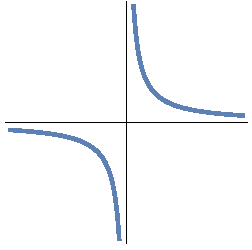
\includegraphics[width=\linewidth]{figures/real-hyperbola.pdf}}
  \noindent 在代数闭域上, 这来自 $xy-1$ 不可约这一事实. 不过, 也可以证明 $X$ 在任意无限域上不可约, 其中包括 $\mathbb{R}$ (Exercise~\ref{ex:hyperbola-irreducible-over-infinite-field}).

  那么, 这个例子中我们的直觉为什么失灵了呢? 答案是 $\mathbb{R}$ 上的解并未反映全貌. 如果拓宽视野, 考虑 $xy-1$ 在 $\mathbb{R}$ 的代数闭包即 $\mathbb{C}$ 上的零点, 就会发现这两\textquotedbl{}块\textquotedbl{}实际上通过复数解相连接. 例如, 可以沿着复数解集
  \[
    \{(e^{\pi\mathrm{i}\theta},e^{-\pi\mathrm{i}\theta})\mid\theta\in[0,1]\}
  \]
  从上面一块中的点 $(1,1)$ 走到下面一块中的点 $(-1,-1)$.

  \BookPairedFigure
    {受这一观察启发, 我们试画 $\mathcal{V}(xy-1)\subseteq\mathbb{A}^{2}_{\mathbb{C}}$. 这有些困难, 因为 $\mathbb{A}^{2}_{\mathbb{C}}$ 在实数上是四维的: $\mathbb{A}^{2}_{\mathbb{C}}=\mathbb{C}^{2}=\mathbb{R}^{4}$. 不过, 通过映入 $\mathbb{R}^{3}$, 可以说明 (Exercise~\ref{ex:complex-hyperbola-real-surface}) 复数解可以与\hyperref[fig:complex-hyperbola]{右图}中的曲面对应起来. 图中还画出了实双曲线和连接 $(1,1)$ 与 $(-1,-1)$ 的路径.}
    {\phantomsection\label{fig:complex-hyperbola}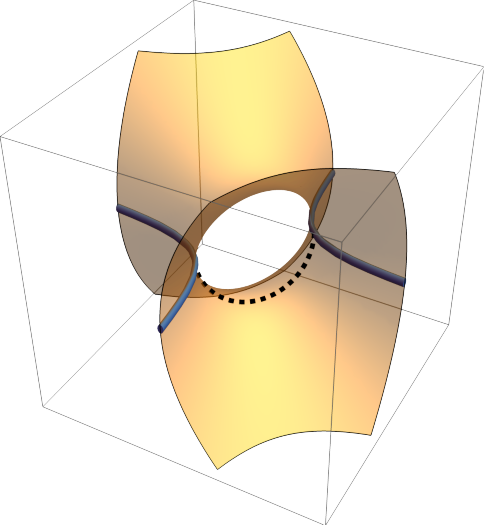
\includegraphics[width=\linewidth]{figures/complex-hyperbola.png}}
  \noindent 因此, 复数情形的图像更接近我们直观上所预期的不可约簇: 它只由一\textquotedbl{}块\textquotedbl{}组成.

  这个例子说明, 在代数几何中利用 $\mathbb{R}$ 上的几何直觉固然重要, 但这样做未必能看到全貌. 只有在能用代数论证加以证明的范围内, 才应当信赖这一直觉.
\end{Example}

有一类特殊的不可约仿射簇只由一个点组成: $X=\{a\}\subseteq\mathbb{A}^{n}$. 由于单点在簇中 (按包含关系) 是极小的, 而 $\mathcal{V}$ 和 $\mathcal{I}$ 算子反转包含关系, 这暗示单点的消没理想应是极大理想. 已知极大理想是特殊的素理想. 这一猜想确实成立, 而且还能说得更多.

\begin{Proposition}{单点与极大理想}\leavevmode\label{prop:single-points-and-maximal-ideals}
  设 $I\subseteq K[x_{1},\ldots,x_{n}]$ 是一个理想. 下列条件等价.
  \begin{enumerate}[label=(\roman*),ref=(\roman*)]
    \item\label{item:maximal-ideal-as-vanishing-ideal-of-singleton} 对某个点 $a=(a_{1},\ldots,a_{n})\in\mathbb{A}^{n}$, 有 $I=\mathcal{I}(\{a\})$.
    \item\label{item:maximal-ideal-as-coordinate-differences} 对某些 $a_{1},\ldots,a_{n}\in K$, 有 $I=\langle x_{1}-a_{1},\ldots,x_{n}-a_{n}\rangle$.
    \item\label{item:maximal-ideal-quotient-is-k} $K[x_{1},\ldots,x_{n}]/I\cong K$.
    \item\label{item:maximal-ideal-condition} $I$ 是极大理想.
  \end{enumerate}
\end{Proposition}

\begin{Proof}
  \ref{item:maximal-ideal-as-vanishing-ideal-of-singleton} 蕴含 \ref{item:maximal-ideal-as-coordinate-differences} 是 Exercise~\ref{ex:vanishing-ideal-of-a-single-point}. \ref{item:maximal-ideal-as-coordinate-differences} 蕴含 \ref{item:maximal-ideal-quotient-is-k} 是 Exercise~\ref{ex:quotient-evaluation-at-point}. \ref{item:maximal-ideal-quotient-is-k} 蕴含 \ref{item:maximal-ideal-condition} 可由 Proposition~\ref{prop:prime-maximal-quotient-characterization} 得出. 因此只需证明 \ref{item:maximal-ideal-condition} 蕴含 \ref{item:maximal-ideal-as-vanishing-ideal-of-singleton}. 假设 $I$ 是极大理想. 由于极大理想都是根理想, 零点定理蕴含 $I=\mathcal{I}(\mathcal{V}(I))$. 要证明 \ref{item:maximal-ideal-as-vanishing-ideal-of-singleton}, 必须证明 $\mathcal{V}(I)$ 是单点. 反设 $\mathcal{V}(I)$ 不是单点. 有两种情形: $\mathcal{V}(I)=\varnothing$ 或 $\mathcal{V}(I)$ 含不止一个点. 若 $\mathcal{V}(I)=\varnothing$, 则
  \[
    I=\mathcal{I}(\mathcal{V}(I))=K[x_{1},\ldots,x_{n}],
  \]
  与 $I$ 的极大性矛盾. 另一方面, 若 $\mathcal{V}(I)$ 含不止一个点, 任取点 $a\in\mathcal{V}(I)$, 并注意 $\varnothing\subsetneq\{a\}\subsetneq\mathcal{V}(I)$ 是仿射簇的严格包含关系. 应用 Proposition~\ref{prop:operators-reverse-inclusions}, 得到
  \[
    K[x_{1},\ldots,x_{n}]\supsetneq\mathcal{I}(\{a\})
      \supsetneq\mathcal{I}(\mathcal{V}(I))=I,
  \]
  这也与 $I$ 的极大性矛盾.
\end{Proof}

注意, \ref{item:maximal-ideal-quotient-is-k} 与 \ref{item:maximal-ideal-condition} 的等价性是纯代数陈述, 在非代数闭域上不成立. 例如, 理想 $\langle x^{2}+1\rangle$ 在 $\mathbb{R}[x]$ 中是极大的, 尽管
\[
  \mathbb{R}[x]/\langle x^{2}+1\rangle\cong\mathbb{C}\not\cong\mathbb{R}.
\]
这一观察反映出 $\langle x^{2}+1\rangle\subseteq\mathbb{R}[x]$ 不是消没理想.

本节最后, 我们描述一部更细致的理想与簇之间的词典. 如前所见, 零点定理蕴含 $\mathcal{V}$ 算子给出 $K[x_{1},\ldots,x_{n}]$ 中的根理想与 $\mathbb{A}^{n}$ 中的仿射簇之间的双射, 其逆是 $\mathcal{I}$ 算子 (Corollary~\ref{cor:radical-ideals-affine-varieties-bijection}). 现在进一步细化这一双射, 把素理想和极大理想也包括进来.

\begin{Proposition}{理想与簇之间更细致的词典}\leavevmode\label{prop:refined-ideals-varieties-dictionary}
  算子 $\mathcal{V}$ 和 $\mathcal{I}$ 是互为逆映射并反转包含关系的双射, 它们建立了下列理想层次与簇的层次之间的对应:
  \[
    \begin{array}{c@{\quad}c@{\quad}c}
      \{K[x_{1},\ldots,x_{n}]\text{ 中的根理想}\}&\longleftrightarrow&
         \{\mathbb{A}^{n}\text{ 中的仿射簇}\}\\
      \rotatebox[origin=c]{90}{$\subseteq$}&&\rotatebox[origin=c]{90}{$\subseteq$}\\
      \{K[x_{1},\ldots,x_{n}]\text{ 中的素理想}\}&\longleftrightarrow&
         \{\mathbb{A}^{n}\text{ 中的不可约簇}\}\\
      \rotatebox[origin=c]{90}{$\subseteq$}&&\rotatebox[origin=c]{90}{$\subseteq$}\\
      \{K[x_{1},\ldots,x_{n}]\text{ 中的极大理想}\}&\longleftrightarrow&
         \{\mathbb{A}^{n}\text{ 中的点}\}.
    \end{array}
  \]
\end{Proposition}

\begin{Proof}
  若 $I$ 是根理想且 $X=\mathcal{V}(I)$, 则零点定理蕴含 $I=\mathcal{I}(X)$. 因此, 根理想与仿射簇之间的双射反转包含关系, 正是 Proposition~\ref{prop:operators-reverse-inclusions} 中的最后一个断言. 要证明 $\mathcal{V}$ 和 $\mathcal{I}$ 限制后给出素理想与不可约簇之间的双射, 只需注意 $I=\mathcal{I}(X)$ 是素理想当且仅当 $X=\mathcal{V}(I)$ 不可约 (Proposition~\ref{prop:irreducible-iff-vanishing-ideal-prime}). 要证明 $\mathcal{V}$ 和 $\mathcal{I}$ 限制后给出极大理想与单点之间的双射, 只需注意 $I=\mathcal{I}(X)$ 是极大理想当且仅当 $X=\mathcal{V}(I)$ 是单点 (Proposition~\ref{prop:single-points-and-maximal-ideals}).
\end{Proof}

\BookExerciseHeading
\begin{BookExercises}
  \item\label{ex:affine-space-is-irreducible} 证明仿射空间在任意无限域上都是不可约的.
  \item\label{ex:irreducible-varieties-over-finite-fields} 说明为什么有限域 (它不可能是代数闭域) 上的仿射簇不可约当且仅当它只含一个点.
  \item\label{ex:coordinate-axes-variety-reducible} 证明 $\mathcal{V}(xy)\subseteq\mathbb{A}^{2}$ 可约.
  \item\label{ex:irreducible-variety-in-finite-union} 设 $X$ 是不可约仿射簇, 并假设
    \[
      X=\bigcup_{i=1}^{r}X_{i},
    \]
    其中每个 $X_{i}$ 都是仿射簇. 证明对某个 $i$, 有 $X=X_{i}$.
  \item\label{ex:sum-of-squares-real-and-complex-irreducibility} 证明仿射簇 $\mathcal{V}(x^{2}+y^{2})\subseteq\mathbb{A}^{2}$ 在 $\mathbb{R}$ 上不可约, 但在 $\mathbb{C}$ 上可约.
  \item\label{ex:real-irreducible-polynomial-with-reducible-variety} 考虑函数 $f=(x^{2}+1)(x^{2}-1)^{2}+y^{2}\in\mathbb{R}[x,y]$.
    \begin{enumerate}[label=(\alph*)]
      \item 用 Eisenstein 判别法证明 $f$ 不可约.
      \item 证明 $\mathcal{V}(f)$ 可约, 由两个不同的点组成.
    \end{enumerate}
  \item\label{ex:hyperbola-irreducible-over-infinite-field} 设 $K$ 是无限域. 本题证明
    \[
      X=\mathcal{V}(xy-1)\subseteq\mathbb{A}^{2}_{K}
    \]
    的不可约性.
    \begin{enumerate}[label=(\alph*)]
      \item 利用 $\mathcal{I}$ 和 $\mathcal{V}$ 的性质证明 $\mathcal{I}(X)\supseteq\langle xy-1\rangle$.
      \item 证明 $\mathcal{I}(X)\subseteq\langle xy-1\rangle$, 可以采用以下策略.
        \begin{enumerate}[label=\roman*.]
          \item 设 $f\in\mathcal{I}(X)$. 证明对某些 $k\in\mathbb{N}$ 和 $g\in K[x]$, 有
          \[
            x^{k}f-g\in\langle xy-1\rangle.
          \]
          \item 利用 $f\in\mathcal{I}(X)$, 证明 $g$ 是零多项式.
          \item 利用 $x^{k}f\in\langle xy-1\rangle$, 证明 $f\in\langle xy-1\rangle$.
        \end{enumerate}
      \item 证明 $\langle xy-1\rangle$ 是素理想, 并用这一点说明为什么 $X$ 不可约.
    \end{enumerate}
  \item\label{ex:complex-hyperbola-real-surface} Example~\ref{ex:hyperbola-is-irreducible} 中画的曲面是实仿射簇
    \[
      Y=\mathcal{V}(uv+w^{2}-1)\subseteq\mathbb{A}^{3}_{\mathbb{R}}.
    \]
    设 $X=\mathcal{V}(xy-1)\subseteq\mathbb{A}^{2}_{\mathbb{C}}$.
    \begin{enumerate}[label=(\alph*)]
      \item 证明 $X=\{(re^{\mathrm{i}\theta},(re^{\mathrm{i}\theta})^{-1})\mid r\in\mathbb{R}_{>0},\ 0\leq\theta<2\pi\}$.
      \item 定义函数 $F:X\to\mathbb{A}^{3}_{\mathbb{R}}$, 把 $(re^{\mathrm{i}\theta},(re^{\mathrm{i}\theta})^{-1})\in X$ 送到
        \[
          \left(\frac{r^{2}-1}{2r}+\frac{r^{2}+1}{2r}\cos\theta,\
            \frac{1-r^{2}}{2r}+\frac{r^{2}+1}{2r}\cos\theta,\
            \frac{r^{2}+1}{2r}\sin\theta\right).
        \]
        证明 $F$ 是从 $X$ 到 $Y$ 的双射.
    \end{enumerate}
\end{BookExercises}

\par\smallskip
{\footnotesize
\noindent\textbf{开放获取.} 本章按照
\href{http://creativecommons.org/licenses/by-nc/4.0/}{Creative Commons Attribution-NonCommercial 4.0 International License}
的条款授权. 该许可允许以任何媒介或格式进行非商业性使用, 分享, 改编, 分发和复制, 但须对原作者和来源作适当署名, 提供 Creative Commons 许可的链接, 并说明是否作了修改.

\noindent
\begin{minipage}[t]{.17\linewidth}
  \vspace{0pt}
\includegraphics[width=.9\linewidth]{figures/source-cc-by-nc.png}
\end{minipage}\hfill
\begin{minipage}[t]{.81\linewidth}
  \vspace{0pt}本章的图片或其他第三方材料均纳入本章的 Creative Commons 许可, 除非材料的署名行另有注明. 如果材料未纳入本章的 Creative Commons 许可, 且您拟进行的使用未获法律规定的许可或超出允许使用的范围, 则须直接向著作权持有人取得许可.
\end{minipage}\par}
